\RequirePackage{luatex85,shellesc}
\documentclass[tikz, multi=false, preview]{standalone}
\usepackage{pgfplots}
\usetikzlibrary{decorations.text}
\usepackage{tikz}
\usepackage{tabularx}
\usepackage[sfdefault]{FiraSans}
\usepgfplotslibrary{units}

\usetikzlibrary{positioning, calc, shapes, arrows, arrows.meta}

\pgfplotsset{
    , xtick align=center
    , ytick align=center
    , unit markings=parenthesis
    , legend style={fill=none,draw=none 
        , font=\footnotesize,at={(0.5,1)}, anchor=south west
    }
    , legend columns = 2
    , axis lines=left
    , ylabel near ticks
}

\begin{document}

\begin{tabularx}{13.5cm}{X X}
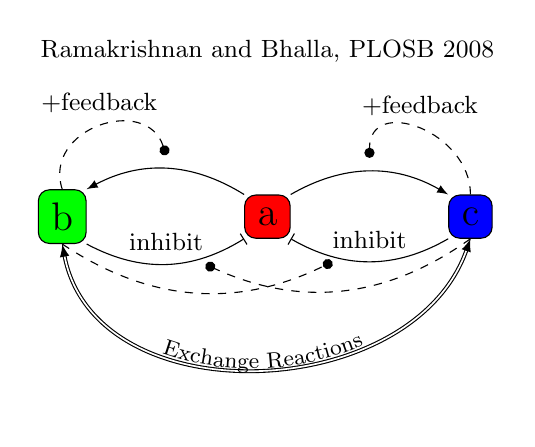
\begin{tikzpicture}[baseline, scale=1, every node/.style={}
    , every edge/.style={very thick}
    ]
    \Large

    \node[minimum size=0.5cm, rounded corners, draw, fill=green] (b) {b};
    \node[minimum size=0.5cm, rounded corners, draw, fill=red, right=2cm of b] (a) {a};
    \node[minimum size=0.5cm, rounded corners, draw, fill=blue, right=2cm of a] (c) {c};

    \draw[-|] (b.south east) to[bend right] 
        node[above, midway] (inhb) {\small inhibit} (a.south west);

    \draw[latex-] (b.north east) to[bend left] 
        node[above, midway] (prodb) {} (a.north west);

    \draw[|-] (a.south east) to[bend right] 
        node[above, midway] (inhc) {\small inhibit} (c.south west);

    \draw[-latex] (a.north east) to[bend left] 
        node[above, midway] (prodc) {} (c.north west);

    % Now c and b catalyze their production.
    \draw[-Circle, dashed] (b.south) to[bend right] 
        node[above, midway] {} (inhc);

    \draw[-Circle, dashed] (b.north) to[bend left,out=90,in=90,looseness=1.5] 
        node[above, midway] {\small +feedback} (prodb.center);


    \draw[-Circle, dashed] (c.north) to[out=90,in=90,looseness=1.5] 
        node[above, midway] {\small +feedback} (prodc.center);

    \draw[-Circle, dashed] (c.south) to[bend left] 
        node[above, midway] {} (inhb);

    % Exchange reaction
    \draw[latex-latex, double
        , postaction={decorate
            , decoration={
                text along path, text={|\footnotesize|Exchange Reactions}
                , text align=center
            }
        }] (b.south) to[bend right, looseness=1.1 , out=-80, in=-110] 
        (c.south);

    % credit
    \node[above=1.5cm of a] {\small Ramakrishnan and Bhalla, PLOSB 2008};
\end{tikzpicture}
&
\begin{tikzpicture}[scale=1
    ]
    \begin{axis}[ 
        , ylabel=Conc
        , width = 6cm, height = 3cm, 
        , enlargelimits = true
        , title = {\small Deterministic}
        ]
    \addplot+ [no marks, very thick] gnuplot [ raw gnuplot ] {
        set datafile separator ',';
        plot "./bistable/gsl.csv" using "time":"c.Co";
    };
    \addplot+ [no marks, very thick] gnuplot [ raw gnuplot ] {
        set datafile separator ',';
        plot "./bistable/gsl.csv" using "time":"b.Co";
    };
    \legend{c, b}
    \end{axis}
\end{tikzpicture}

\begin{tikzpicture}[scale=1
    ]
    \begin{axis}[ 
        xlabel=Time, x unit=sec
        , ylabel=Conc
        , width = 6cm, height = 3cm, 
        , enlargelimits = true
        , title = {\small Stochastic}
        ]
    \addplot+ [no marks] gnuplot [ raw gnuplot ] {
        set datafile separator ',';
        plot "./bistable/gssa.csv" using "time":"c.Co";
    };
    \addplot+ [no marks] gnuplot [ raw gnuplot ] {
        set datafile separator ',';
        plot "./bistable/gssa.csv" using "time":"b.Co";
    };
    \legend{c, b}
    \end{axis}
\end{tikzpicture}
\end{tabularx}
\end{document}

